%\subsection{Histogramm f\"ur Property (299)}
%\begin{figure}
\begin{center}
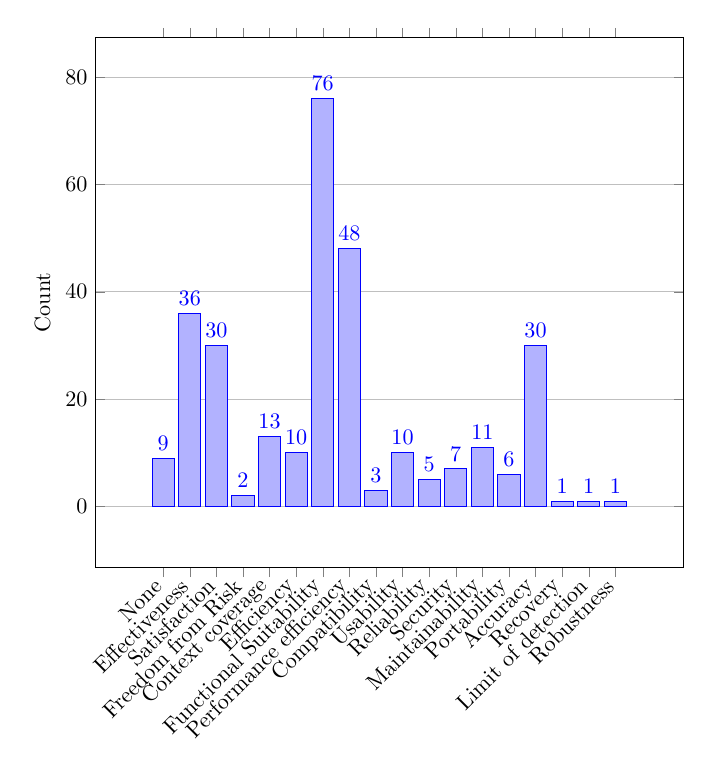
\begin{tikzpicture}[scale=.8]
\begin{axis}[ ybar, ymajorgrids, enlargelimits=0.15, legend style={at={(0.5,-0.15)}, anchor=north,legend columns=-1},
    width=.90\linewidth,height=10cm,
    nodes near coords, %nodes near coords align=below,
    ylabel={Count}, ymin=0,
    x tick label style={rotate=45,anchor=east},
    xtick={1,2,3,4,5,6,7,8,9,10,11,12,13,14,15,16,17,18},
    xticklabels={None,Effectiveness,Satisfaction,Freedom from Risk,Context coverage,Efficiency,Functional Suitability,Performance efficiency,Compatibility,Usability,Reliability,Security,Maintainability,Portability,Accuracy,Recovery,Limit of detection,Robustness
}
    %xlabel={Property}    
    ]
  \addplot coordinates { (1,9)  (2,36)  (3,30)  (4,2)  (5,13)  (6,10)  (7,76)  (8,48)  (9,3)  (10,10)  (11,5)  (12,7)  (13,11)  (14,6)  (15,30)  (16,1)  (17,1)  (18,1)   };
\end{axis}
\end{tikzpicture}
\end{center}
%\caption{Histogramm f\"ur Property (299)}
%\label{fig:histo_property}
%\end{figure}

